
\documentclass[a4paper]{article}
 
% A simple Latex document illustrating some of the main document features

\usepackage{natbib}
\usepackage{graphicx}
\usepackage{pdfpages}

\usepackage{setspace}
\usepackage{textcmds}

\begin{document}

\title{Data Mining Coursework}
\author{Olajumoke Akinremi / 100432440}
\date{May 2024} % Leave this empty if you prefere
\maketitle

\section*{Abstract}
Machine Learning (ML) has emerged as a significant trend within the technologically advanced industrial sector. The influence of ML techniques can be seen across various fields, including the medical, industrial, and security sectors. ML possesses the capability to identify patterns in data and can also predict diseases using medical information sources\citep{tumpa2022review}. Initially, the dataset was cleaned and then divided into a validation dataset. Various approaches, including the use of imbalanced and balanced datasets, were implemented. The use of random forest classifier with parameters n\_estimators= n 100 resulted gave the best classifier. 


\section{Introduction} \label{intro}

Supervised Classification aims to develop classification rules with minimal classification cost. It can be viewed as an optimization problem \citep{silva2017optimization}
 This coursework specifically addresses multi-class classification, involving the categorization of more than two attributes. With the progression of technology, the healthcare sector has similarly advanced. Within healthcare, the development of models capable of pinpointing patient conditions with utmost accuracy holds significant value. Such precision facilitates the timely provision of necessary treatment to the appropriate patients, thereby mitigating instances of occurrence, relapse, and even mortality in certain scenarios. Hence, the significance of the tasks outlined in this coursework is paramount. 

The dataset comprises anonymized data from 4,250 records, including 24 columns related to demographic information, health status indicators, and results from various medical tests. Key attributes encompass age, gender, sick, pregnant, concern\_type1,concern\_type2, enlargement, tumor, disorder, medication\_A,medication\_B, mental\_health,mood\_stabiliser, surgery,treatment\_type1, suspect,test\_X1,test\_X2,test\_X3,test\_X4,test\_X5,test\_X6. This diverse dataset presents an opportunity to apply data mining tools and techniques, uncovering hidden patterns and relationships.

Our analysis focuses on understanding the underlying data structure comprehensively, address challenges like missing values and outliers, and utilize both supervised to make predictions and compare the result with alongside unsupervised learning methods. The insights gained from this project could impact real-world healthcare practices by offering a methodological framework for disease risk prediction and patient categorization.



\section{Data Exploration, Visualisations, and Summary}
\subsection{Data Exploration}
 The data exploration stage is a critical stage as it aims to reveal insights about the data’s composition and quality. Our primary objectives include observation of the features in the healthcare dataset, detecting missing values and outliers, and visually exploring data distributions and variable relationships. 
 
 Firstly, Panda was utilized to load the dataset and upon loading the data into the Jupiter notebook, it was observed that the dataset has a total of 4250 instances and 24 attributes Subsequently, we present the initial 5 rows and the last 5 rows of the dataset to gain an initial understanding of its structure and have a feel of the dataset. 
 \subsection{Summary}
 A summary of the dataset shows that the dataset consists of 17 categorical and 7 numerical data types. The categorical data type includes gender, sick, pregnant, concern\_type1,concern\_type2, enlargement, tumor, disorder, medication\_A,medication\_B, mental\_health,mood\_stabiliser, surgery, treatment\_type1 and 
 suspect while the numerical data type includes : 
 age, test\_X1, test\_X2, test\_X3, test\_X4, test\_X5, test\_X6. 
 
 The descriptive statistics for both categorical and numerical data were analyzed to provide insights into the dataset’s central tendencies, dispersion, and distribution shape as shown in Figure \ref{fig:cat} and Figure \ref{fig:num}. The dataset was categorized into numerical and categorical data to enhance understanding of these statistics. Looking at the standard deviation, it can be assumed that age, test\_X1,test\_X3 and test\_X5 have high values of 1004.518, 32.657, 35.496, and 39.837 respectively. It can be assumed that these records would have a high impact on our prediction and further investigation would be done to verify the assumptions.
\begin{figure}
    \centering
    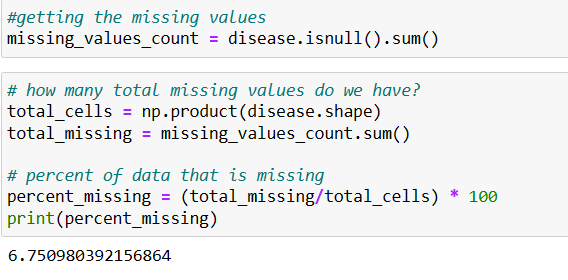
\includegraphics[width=0.5\linewidth]{missing_value.png}
    \caption{Percentage Missing Value}
    \label{fig:missing}
\end{figure}
For the numerical data type, missing values were noted in all variables except for age while for categorical data, only gender has missing values of 141. Additionally, outliers were identified in variables such as age and all the test\_X, with age as high as 65526 being recorded, which seems unrealistic. This will be further investigated to verify the assumption.
\begin{figure}
    \centering
    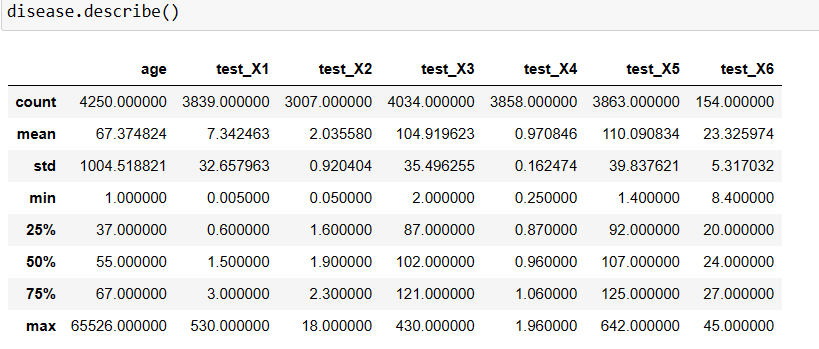
\includegraphics[width=0.5\linewidth]{describe.png}
    \caption{Summary of the numerical variables}
    \label{fig:num}
\end{figure}
\begin{figure}
    \centering
    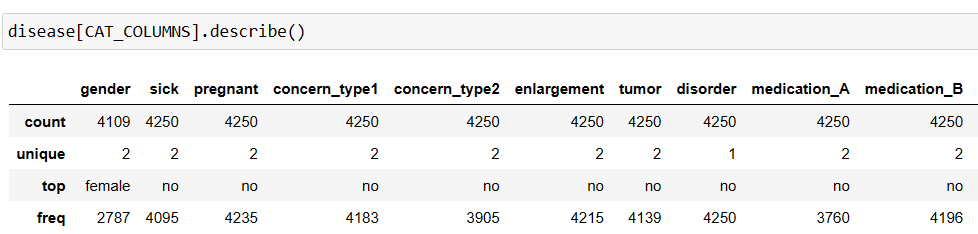
\includegraphics[width=0.5\linewidth]{categorical.png}
    \caption{Summary of the Categorical variables}
    \label{fig:cat}
\end{figure}
\begin{figure}
    \centering
    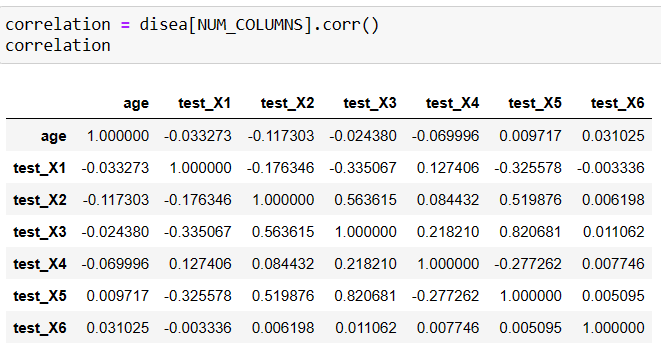
\includegraphics[width=0.5\linewidth]{correlation.png}
    \caption{Correlation}
    \label{fig:correla}
\end{figure}
Regarding the categorical variables, it appears that the health disease in question predominantly affects females, who constitute 67\% of the dataset, with males accounting for 31\% and the remaining 2\% representing missing values. Of the 2787 females in the dataset, 15 were reported as pregnant. Only 104 females are classified as high risk, 2,324 as low risk, and 359 as moderate risk. Among these 104 high-risk females, only one reported being pregnant. This suggests that the disease is likely not related to pregnancy as shown in \ref{fig:preg}. Out of the total 4250 records, there were 67 cases of Concern\_type 1, 345 of Concern\_type 2, 35 experienced enlargement, 111 had tumors, 490 were on Medication A, 54 on Medication B, 194 had mental health issues, 45 were on mood stabilizers, 62 had undergone surgery, 81 were receiving treatment type 1, and 299 cases were suspected. A table showing the percentage of this occurrence is shown in Figure \ref{fig:percen}
\begin{figure}
    \centering
    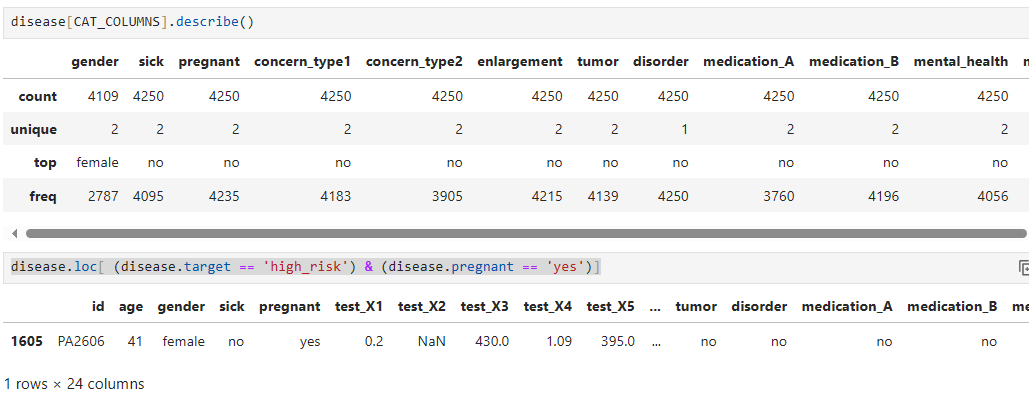
\includegraphics[width=0.5\linewidth]{gender.png}
    \caption{Pregnacy output}
    \label{fig:preg}
\end{figure}
\begin{figure}
    \centering
    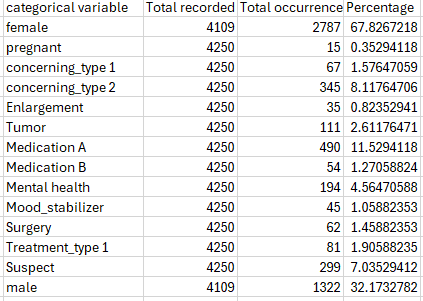
\includegraphics[width=0.5\linewidth]{data_mining_coursework.png}
    \caption{Summary}
    \label{fig:percen}
\end{figure}

\subsection{Missing Values}
Gender is missing 141 values, test\_X1 is missing 411, test\_X2 is missing 1243, test\_X3 is missing 216, test\_X4 is missing 392, test\_X5 is missing 387, and test\_X6 is missing 4096 values. Notably, test\_X6 has over 96\% of its values missing, which could potentially introduce bias and complexity to the model if not addressed. The total percentage of missing values across the entire dataset is 6.75\% as shown in Figure \ref{fig:missing}. Although some missing values are present in all tests, only test\_X6 will be entirely excluded due to the specifics of our data set. This data set pertains to individual health, and what may appear to be an outlier might not be one. 


\subsubsection{Handling of Missing Values}
Regarding imputation methods, zero filling, 'bfill', TransformerMixin were explored and the descriptive statistics of each were examined. The TransformerMixin proved to be the most effective, as it yielded new mean values that closely resembled the original data.
\subsection{Outliers}
A closer examination of the dataset revealed two outliers in the age variable, which were identified as shown in \ref{fig:age}. A close examination of the data set shows that age has maximum value of 455 and 65,526 which is not possible and thus further exploration needs to be performed. Also tests\_X1 has maximum of 530, tests\_X3 has maximum of 430 and tests\_X5 has maximum of 642. However, the outliers in the age variable may be due to errors during imputation and this will be handled by replacing with the median, instead of deleting the whole column. Deleting the outliers in age would further reduce the number of data available.   DBSCAN identified a total of 397 outliers whereas Isolation Forest identified 43 outliers. Adjusting the minimum samples to 2, 3, and 5 resulted in outputs of 301, 397, and 483, respectively. This indicates that selecting a lower value for minimum samples leads to the detection of fewer outliers. Given that the dataset pertains to healthcare, it's unclear whether the outliers in various tests represent patients with significant variations; therefore, these will not be removed. 
\begin{figure}
    \centering
    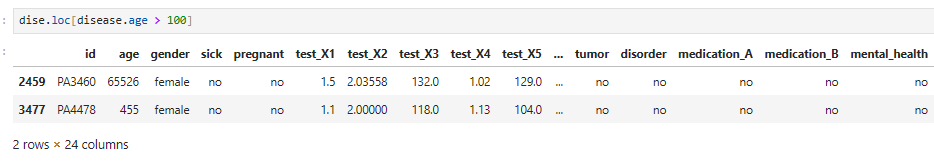
\includegraphics[width=0.5\linewidth]{age.png}
    \caption{Outlier in Age}
    \label{fig:age}
\end{figure}
\subsubsection{Handling of Outliers}
 The median was calculated and it gave a result of 55.0, this was used to replace the two outliers
\subsection{Visualization}

A detailed examination of the scatter plot and data correlation reveals some clustering into two distinct groups. Age has the strong positive correlation with test\_X6. Test X1 is most positively correlated with test X4, while test\_X2 has the highest positive correlation with test\_X3. Test\_X3 had the strongest positive correlation with test\_X5, registering a correlation coefficient of 0.820, which exceeds the threshold of 0.7, suggesting that a model that can handle multicollinearity must be used. Additionally, test\_X4 and test\_X5 both show the highest positive correlations with test\_X3, and test\_X6 is most positively correlated with age.
The analysis reveals an uneven distribution of risk categories among the targets. Specifically, 3,612 individuals are categorized as low risk, 489 as moderate risk, and 149 as high risk. Consequently, approximately 84\% of patients are at low risk for this specific disease, while around 5.5\% face high risk.

Correlation studies involving numerical columns as shown in Figure \ref{fig:correla} and visualized through heatmap indicate that tests X3 and X5 share a high correlation, with a coefficient of 0.82. The correlation analysis highlighted that test\_X6 lacks any correlation with other tests and, along with the disorder feature

KDE plots suggest shifts in age distributions across risk levels, with individuals aged 0-5 and 45-100 primarily at moderate risk, and those aged 25-45 at high risk. The age distribution exhibits multiple peaks, indicating varied risk categories across different age groups.

Test\_X1 displays considerable variation at moderate risk levels, whereas high-risk categories show a broader spread, particularly for tests\_X3 and test\_X5, supporting the observed high correlation. They both show the transition in risk levels moves from moderate to low and then to high, with the high-risk category exhibiting a broader spread.Test\_X4 demonstrates variability, with high risk appearing between ranges of 0.0 – 0.75 and 1.70– 2.00. Test\_X6 shows little distinction between risk levels and might be considered for exclusion from the analysis.


Examining the histogram, distinct age brackets are visible: 0-20, 21-40, 41-60, 61-80, and 81-100, which will be utilized for feature engineering. In terms of unique values, age had 92, ID had 4250, and the tests had varying numbers of unique values: X1 had 335, X2 had 78, X3 had 246, X4 had 125, X5 had 264, and X6 had 26. While the unique values for tests X1 to X6 will remain unchanged due to insufficient test information, age will be regrouped into the aforementioned brackets.

When comparing gender with the target, it is apparent that the disease disproportionately affects females more than males. Analysis of the 'sick' status with the target showed that most individuals who reported not being sick were at low risk, but a notable fraction were at high risk—unlike those who reported being sick, all of whom were at low risk. The comparison with pregnancy status indicated that while most non-pregnant individuals were at low risk, a significant number were at high risk, suggesting the disease is not related to pregnancy.

The analysis also concluded that individuals who underwent treatment type 1, surgery, or are currently on mood stabilizers, as well as those with mental health issues, on medication A and B, or with a tumor and reported enlargement, are not at risk of this disease. 

\subsection{Data Cleaning and Pre-processing}
\subsubsection{Data Cleaning}
The patient ID and test\_X6 will be removed from the analysis. The patient ID is irrelevant, and test\_X6 will be excluded because approximately 96\% of its data is missing, which would only complicate the model unnecessarily.
Text\_x5 would be removed as it is highly correlated with test\_X3 and we have a total of 89,250 datasets for our modelling. To prepare the data correctly for modeling, pre-processing steps like Label encoding and One-hot encoding are applied to the dataset. Necessary libraries are imported from pandas and a total of 35 columns were obtained. After this, a feature ranking algorithm was employed to assess all the numeric input features, along with 'y', the output variable still referred to as 'target'. The ranking utilized criteria such as mutual\_info\_classif and f\_classif. It was noted that the rankings from both criteria aligned closely in terms of feature prioritization.
\subsubsection{Data Pre-processing}
To ensure the data is correctly formatted for the model, pre-processing steps like Label encoding,One-hot encoding, and Feature selection are applied to the dataset. Label encoding is used for the target variable and one-hot encoding for the categorical variable. It encoded high risk to 0, low risk to 1, and moderate risk to 2 as shown in \ref{fig:label}. Necessary libraries are imported from pandas. Following this, a feature ranking algorithm is used to evaluate all the features, including numeric input features and the target output variable, y. The ranking employs mutual\_info\_classif and f\_classif criteria, which both yielded consistent results in feature ranking. Ranking evaluation of two feature ranking models revealed a consensus on six(6) of the top ten(10) features: test\_X1, test\_X2, test\_X3,test\_X5,concern\_type 2\_yes,concern\_type 2\_no indicating key areas of focus for further analysis.
\section{Supervised Modeling}

\begin{table}
    \centering
    \begin{tabular}{cccccc}
        Classifer & Accuracy & Precision  & Recall  & Training score  & Test score \\
        knn & 0.90 & 0.92  & 0.90  & 1.00  & 0.9035 \\
        svc & 0.86 & 0.91 & 0.86  & 0.8706 & 0.860 \\
         clf & 0.94 & 0.96 & 0.94 & 0.9370 &  0.9435\\
        rf & 0.988 & 0.99 & 0.99 & 0.9993 & 0.9882 \\
        rf2 & 0.9905 & 0.99 & 0.99  & 1.00  &  0.9906\\
        gb & 0.9905 & 0.99 & 0.99 & 0.9979 & 0.9906 \\
    \end{tabular}
    \caption{Result of supervised modelling}
    \label{tab:my_label}
\end{table}

\subsection{Balancing of  dataset}
Applying the Synthetic Minority Over-sampling Technique (SMOTE) helped balance the dataset, leading to more equitable performance across different classes. This improvement is evident in the subsequent use of the KNN Classifier, Decision Tree Classifier, Random Forest and Gradient Boost.
\begin{figure}
    \centering
    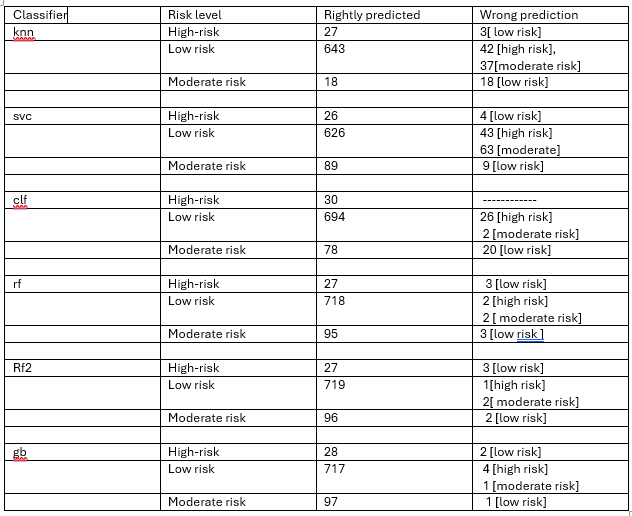
\includegraphics[width=0.5\linewidth]{class.png}
    \caption{Classifiers}
    \label{fig:class}
\end{figure}
\subsubsection{KNNeighbours(knn)}

The model reached its peak average accuracy when k was set to 1, with a mean accuracy of 0.90 indicating that it accurately predicted the class labels for about 90\% of the instances in the cross-validated training dataset. This result suggests that a smaller k value, specifically 1, enhances performance for this training data. It is important to recognize that the optimal k value varies based on the unique attributes of the data, and in this case, a smaller k value proved beneficial for achieving higher accuracy. The recall rate was also 90%.

\subsubsection{SVC(svc)}

The Support Vector Classifier (SVC) achieved an impressive accuracy of 86\%, indicating that it correctly predicts 86\% of the outcomes. Additionally, the precision is also at 91\%, meaning that when the model predicts a positive result, it is correct 91\% of the time. The recall is at 86\%, demonstrating the model's ability to identify 86\% of all actual positives. On the performance of the model on the training Set,the model scores 87.06\% on the training dataset representing the proportion of correct predictions made from the training data while On the test dataset, the accuracy is 86\%, which is close to the training set score. 

The performance degradation of KNN and SVC can be linked to the multicollinearity in the dataset, particularly due to the strong correlation between features X3 and X5, highlighting the necessity for an ensemble approach
\subsubsection{Decision Tree (clf)}

 The model achieves an impressive accuracy of 94\%, indicating its proficiency in correctly predicting outcomes across the dataset.
With a precision of 96\%, the model effectively predicts positive outcomes while minimizing false positives.
The recall rate of 94\% demonstrates the model's ability to identify 94\% of all actual positive cases. For the Dataset Performance, the model achieves an accuracy of 93.7\% on the training dataset, showing strong learning without significant overfitting. On the test dataset, the accuracy is 94.35\%, slightly higher than the training set but still indicative of good generalization to new, unseen data. 

In conclusion, the decision Tree model performs well, with high accuracy, precision, and recall but there is a need for an ensemble to handle high correlation between the features. The consistency between training and test dataset metrics suggests effective generalization beyond the training data. Notably, the 94\% precision highlights the model's ability to minimize false positives.

\subsubsection{Random Forest Classifier(rf)}
 The performance of a Random Forest model under two different configurations was analyzed: one with 10 trees (n=10) and another with 100 trees (n=100). The evaluation focuses on accuracy and the model's effectiveness on the training and test datasets.
 Model Performance with n = 10 Trees
This model achieves a high accuracy of 98.8\%, showcasing strong predictive abilities. It attained a perfect score of 99.93\% on the training set, indicating flawless accuracy during training. However, the test score was slightly lower at 98.82\%, which, while still outstanding, points to a slight degree of overfitting when transitioning from training to real-world application.

 Model Performance with n = 100 Trees
The accuracy has improved to 99.05\%, indicating enhanced performance with the addition of more trees. It sustained a perfect score of 100\%, mirroring the performance of the smaller model. Additionally, there is a slight improvement to 990.6\%, which closely matches the performance seen with the training data..

 The increase in the number of trees from 10 to 100 results in noticeable accuracy improvement, both overall and on the test set. This suggests better generalization and robustness against overfitting.

 In Conclusions, both Random Forest configurations demonstrate exceptional performance, with the 100-tree version having a slight edge in accuracy and generalization. Consistent training scores highlight strong learning capability, while excellent test scores reflect the models' ability to handle new, unseen data effectively.

\subsubsection{Gradient Boost Classifer(gb)}
This report evaluates a Gradient Boosting Classifier that is set up with 100 boosting stages (n=100), focusing on its accuracy and effectiveness across both training and testing datasets.

 Model Performance : 
The classifier achieves an impressive accuracy of 99.05\%, showing a high level of precision in its predictions. With a training score of 99.79\%, the model is almost perfect, demonstrating successful learning from the training data. The test score also stands at 99.06\%, mirroring the overall accuracy, which indicates that the model generalizes exceptionally well to new data and displays minimal signs of overfitting. The high accuracy rate confirms the classifier's effectiveness in making accurate predictions across both known and unknown datasets, highlighting its strong generalization capabilities. The slight difference between the training and test scores suggests that the model effectively handles complexity and is resilient to overfitting, which is especially notable in the context of the high dimensionality and iterative nature of boosting classifiers.

100-stage Gradient Boosting Classifier demonstrates stellar performance, characterized by high accuracy and superior generalization from training data to practical applications. The consistency of the model across various datasets underlines its reliability and predictive strength.

Analyzing the confusion matrix, a random forest classifier with 100 trees accurately identified 27 high-risk cases and misclassified 3 as low-risk. It correctly classified 719 low-risk cases, with errors including 1 misclassified as high risk and 2 as moderate risk. Furthermore, it accurately predicted 96 moderate-risk cases, though 2 were incorrectly labeled as low-risk. This analysis supports the classifier's accuracy.

The tested classifiers exhibit a broad spectrum of accuracy, with ensemble approaches, especially those utilizing boosting techniques, surpassing simpler models. Among these, the Random Forest Classifier with n value 0f 100 stands out as the top performer, reaching the highest accuracy, which highlights the benefits of integrating multiple weak learners to enhance predictive performance.

The test data was loaded into the Jupyter notebook and underwent the required pre-processing. After cleaning, predictions were made using our most effective classifier.
\section{Unsupervised learning}
The pre-processed data, which included the target variable, was utilized for clustering. Unsupervised learning focuses on making predictions without using labeled targets. A pair plot was utilized to examine the associations among the features. Specifically, when analyzing the pair plot of age and test X1, four clusters were apparent, and this observation was subsequently validated using K-means clustering. By applying K-means and silhouette analysis, a K value of 5 was determined, aligning with the observations from the pair plot. Additionally, when considering test\_X1 and test\_X4, three clusters were visible, which also matched the K values derived from K-means and silhouette analysis. Although clustering is useful for revealing relationships between features, it does not provide precise predictions but rather aids in enhancing visualization. Unlike supervised learning, which provided an accurate count of incorrectly predicted outcomes, unsupervised learning offered only visual representations.


\section{Summary/Conclusion}
In the model selection process, the ensemble can handle data with multicollinearity without having to remove the column. Random Forest ensemble for Decision Tree delivered superior results and was chosen for prediction. For future work, alternative methods, such as splitting the dataset prior to applying the models, will be explored to see if there are potential improvements. 

\section{Other resources}
Other resources used for this project include: coursework lectures, coursework lab, Datacamp, Kaggle



\bibliographystyle{plainnat}
\bibliography{name}

\end{document}
